\begin{figure}[!ht]
    \centering
    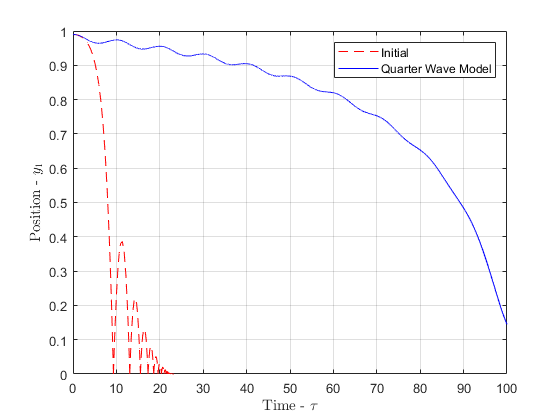
\includegraphics[width=0.4\textwidth]{Figures/QWMSimulation/NearEquilibriumOscillations/Position.png}
    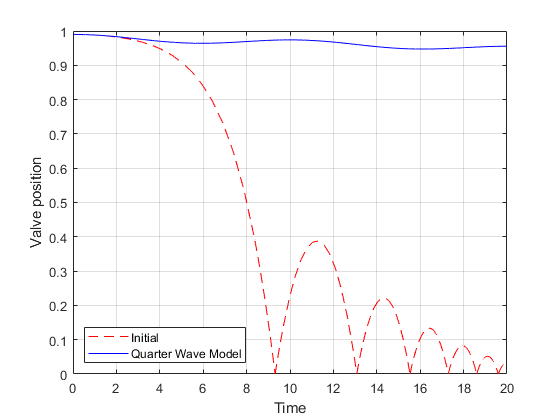
\includegraphics[width=0.4\textwidth]{Figures/QWMSimulation/NearEquilibriumOscillations/Position-Short.png}
    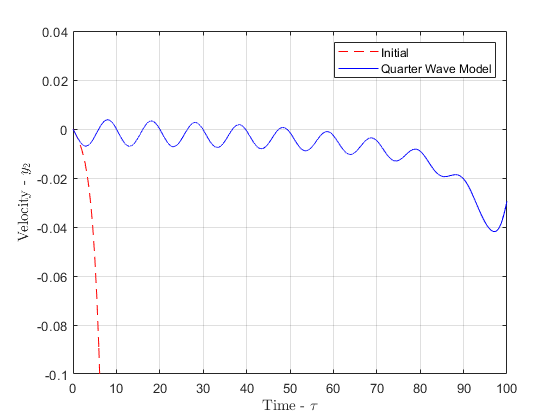
\includegraphics[width=0.4\textwidth]{Figures/QWMSimulation/NearEquilibriumOscillations/Velocity.png}
    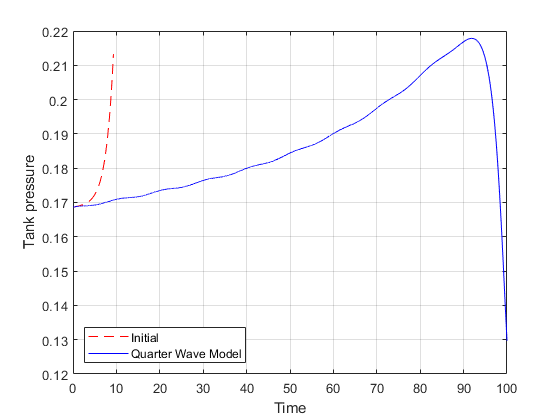
\includegraphics[width=0.4\textwidth]{Figures/QWMSimulation/NearEquilibriumOscillations/Pressure.png}
    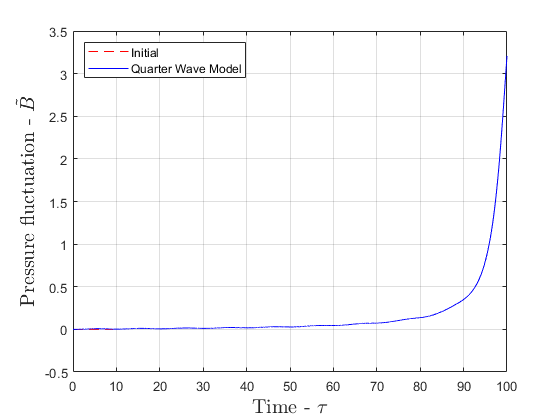
\includegraphics[width=0.4\textwidth]{Figures/QWMSimulation/NearEquilibriumOscillations/B.png}
    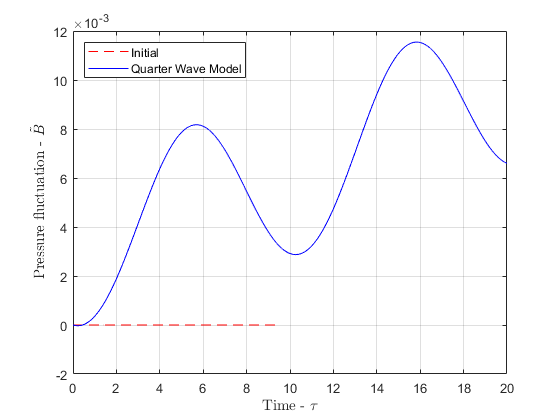
\includegraphics[width=0.4\textwidth]{Figures/QWMSimulation/NearEquilibriumOscillations/B-Short.png}
    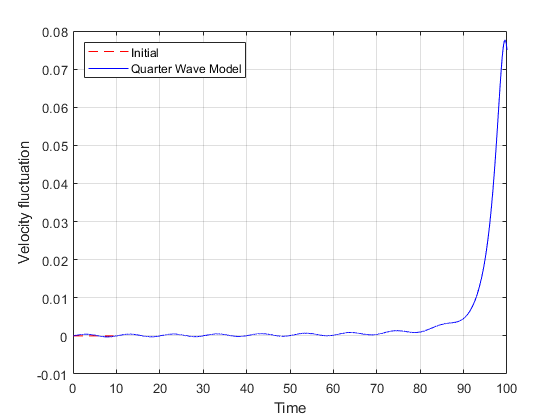
\includegraphics[width=0.4\textwidth]{Figures/QWMSimulation/NearEquilibriumOscillations/C.png}
    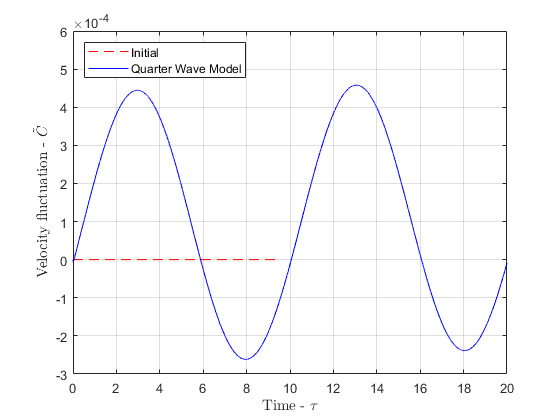
\includegraphics[width=0.4\textwidth]{Figures/QWMSimulation/NearEquilibriumOscillations/C-Short.png}
    \caption{Simulation of QW with $\gamma = 14.9501$, $q = 0.6$, $\Lambda = 0$, $\alpha = 8.5658$, $\delta = 1$, $\kappa = 0$, $\beta = 0$, $\mu = 0.1407$, $\sigma = 10.3808$, $\phi = 0$ and $r = 0.8$. Equilibrium pressure is $p = 0.1686$ but the tank is actually held at $p = 0.0703$. Pressure comes from close to calculated instability boundary.}
    \label{fig: QWNearEquil}
\end{figure}